\documentclass[e4_tp3_main.tex]{subfiles}
\begin{document}
\newgeometry{top=2.5cm, bottom=2.0cm, left=2.25cm, right=2.25cm}

\section{Control de velocidad de motores de inducción trifásicos}
Se procedió a analizar el circuito con el cual se realiza un control sobre un motor trifásico.
\subsection{Análisis a lazo abierto}

\subsubsection{An\'alisis de las señales en el encendido y cuando se aplica un escal\'on de torque}

En esta etapa, vamos a realizar un análisis sobre el circuito a lazo abierto. Para ello, se dispuso del circuito de la siguiente forma:
\begin{figure}[H]
\centering
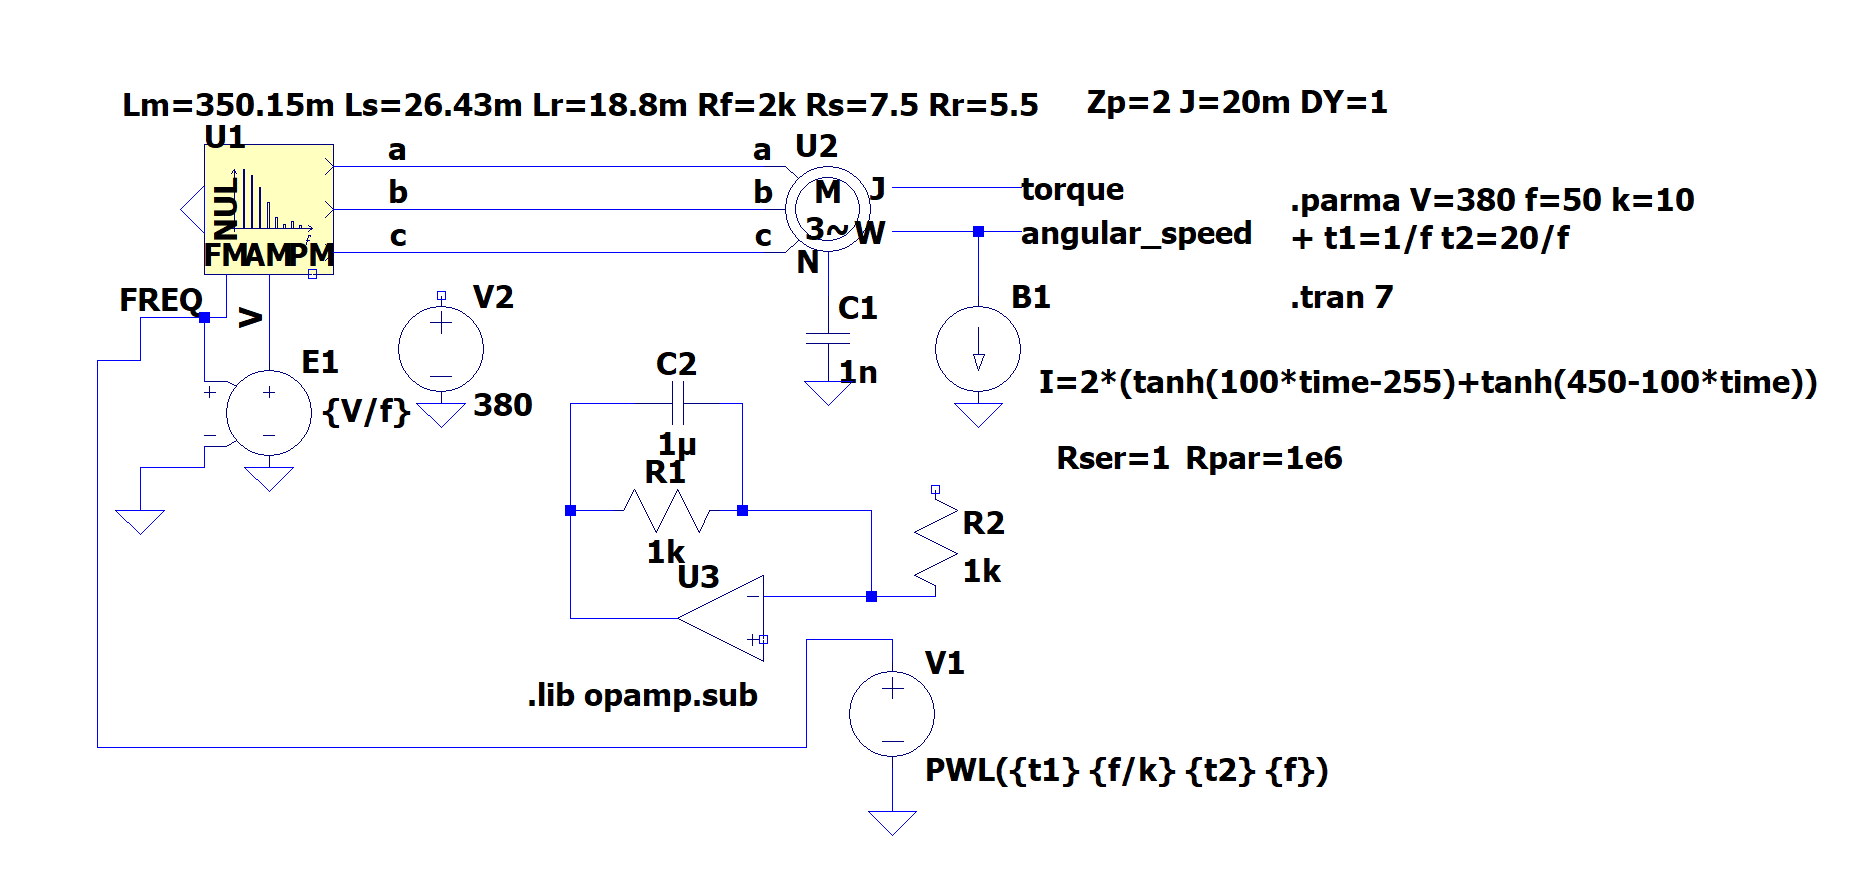
\includegraphics[width=0.7\linewidth]{Imagenes/3-1-a-circuito.png}
\caption{Diagrama del circuito a lazo abierto}
\end{figure}

Una vez configurado el generador con N=2k+1 a fin de insertar los armónicos impares en la tensión de línea, obtuvimos los siguientes resultados:

\begin{figure}[H]
	\centering
	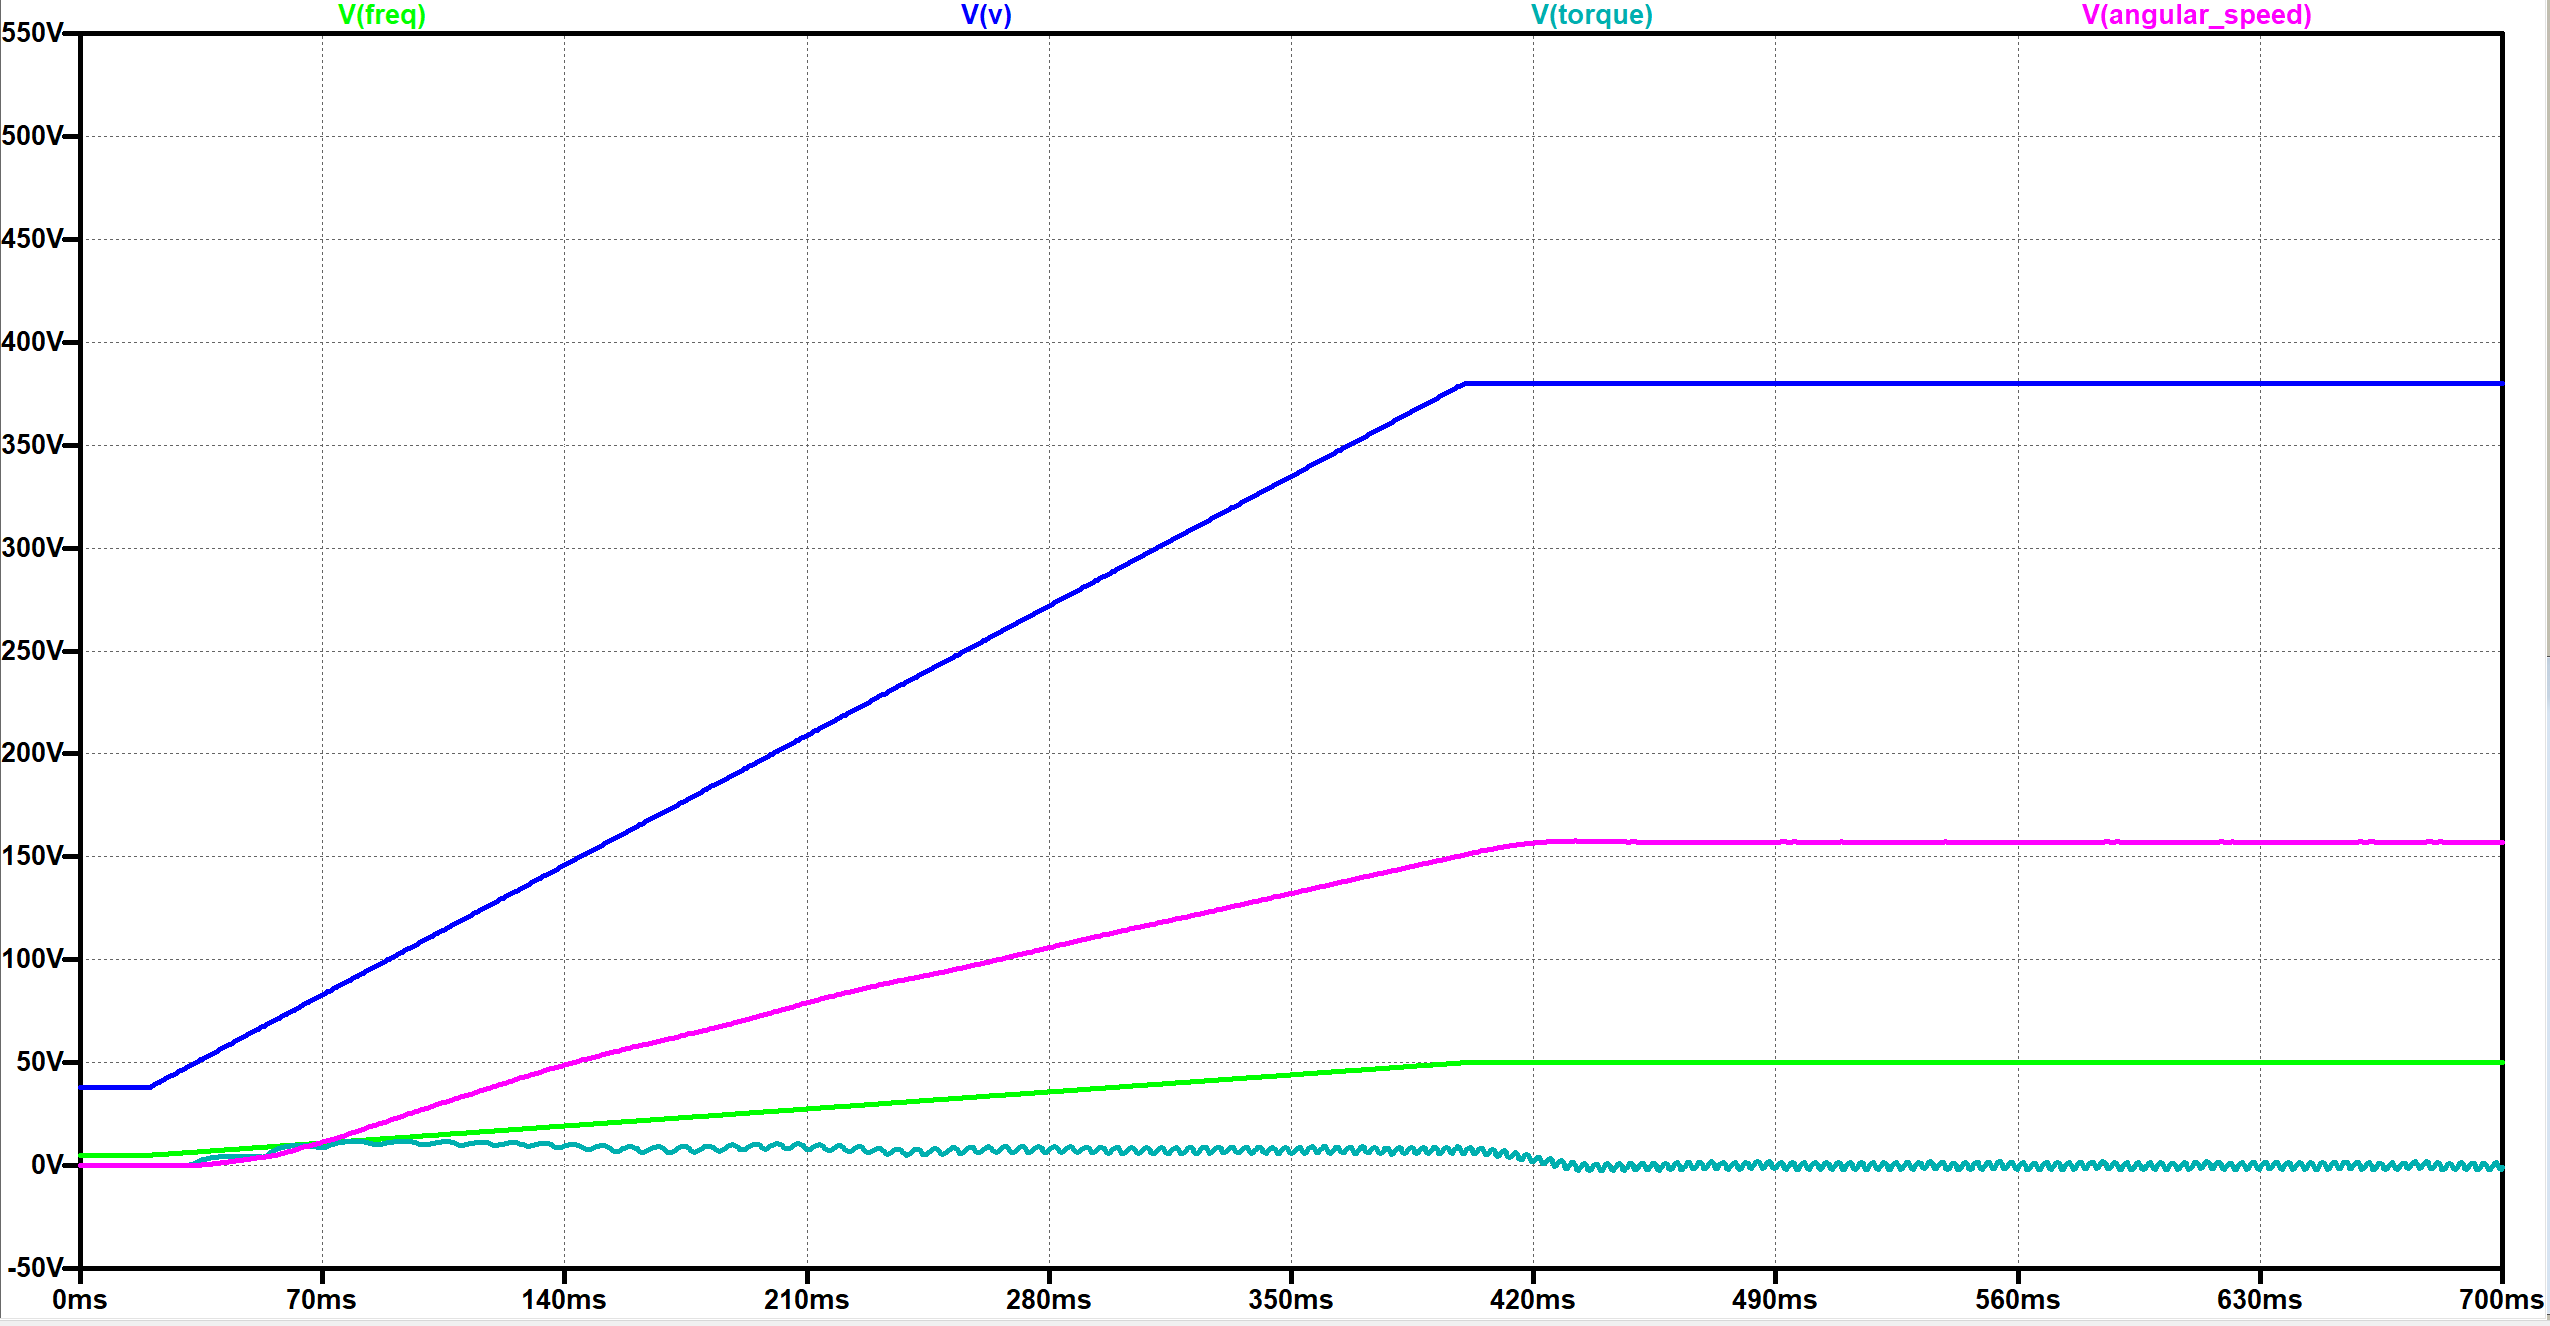
\includegraphics[width=0.6\linewidth]{Imagenes/3-1-a-inicio.png}
	\caption{Simulaci\'on del encendido del circuito}
	\label{fig:enc}
\end{figure}

\begin{figure}[H]
	\centering
	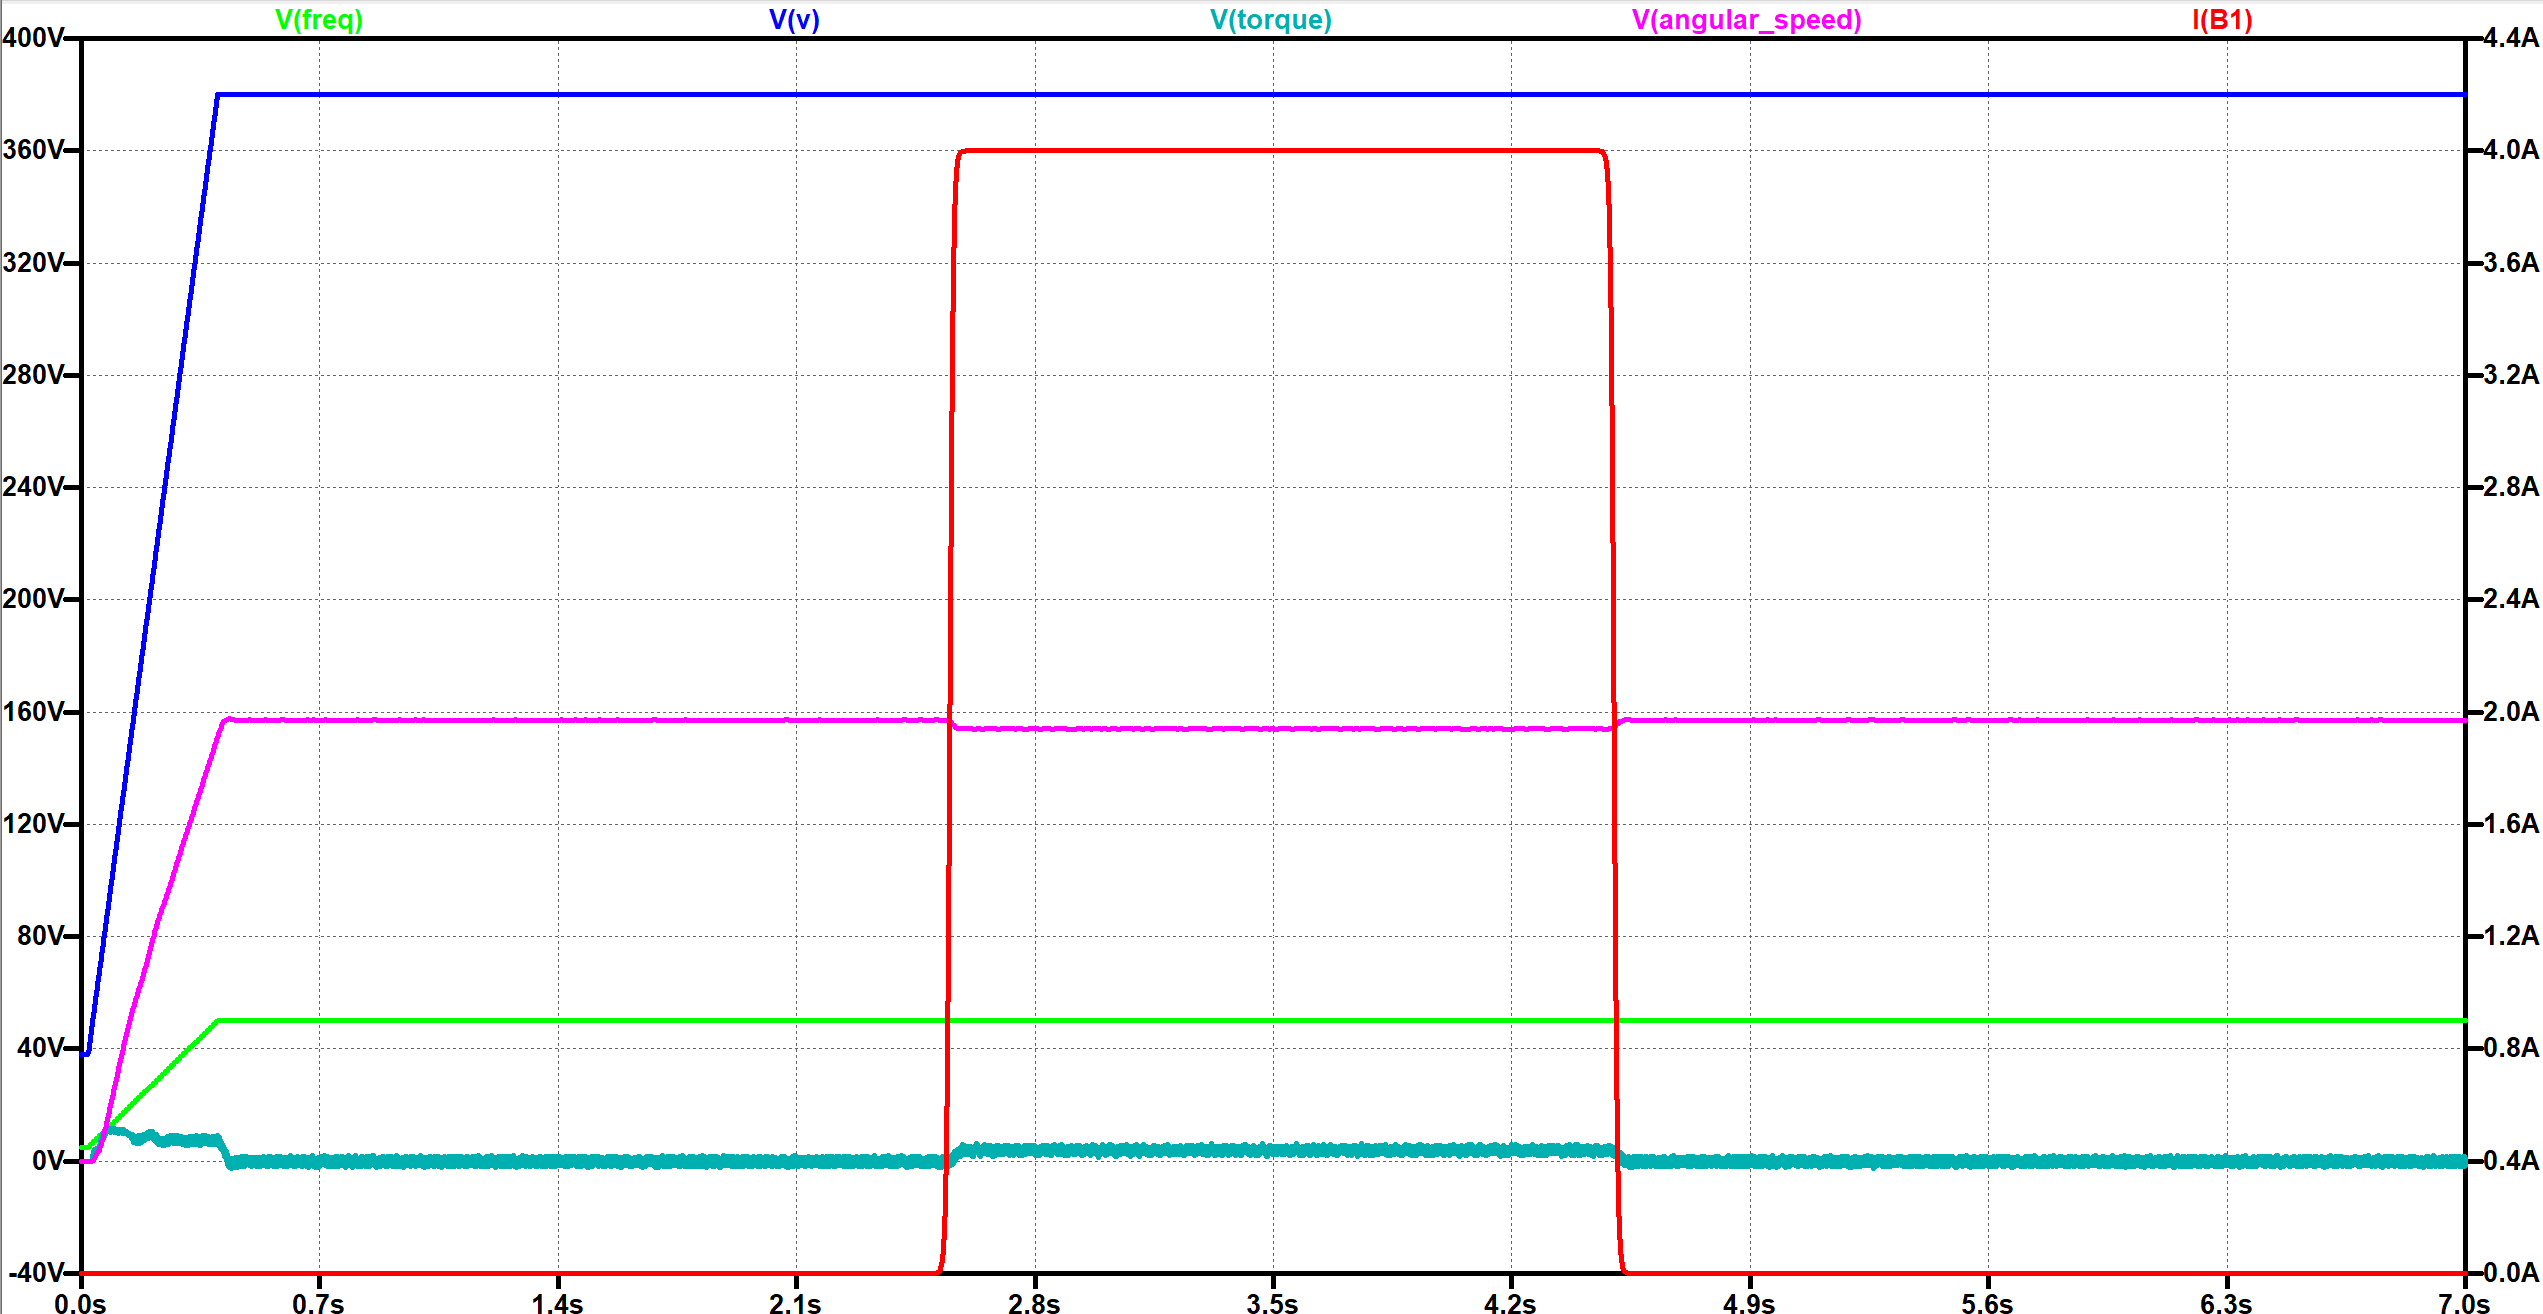
\includegraphics[width=0.6\linewidth]{Imagenes/3-1-a-general.png}
	\caption{Simulación del circuito con esca\'lon de torque}
	\label{fig:torq}
\end{figure}

En la figura podemos observar cómo se comportan las señales de frecuencia del motor $V(freq)$, su velocidad angular $V(angular\_speed)$, el torque $V(torque)$, la carga $I(B)$ y la tensión $V(v)$.
\vspace{0.5cm}

Ni bien se enciende el circuito (Ver Figura \ref{fig:enc}), observamos como la tensión de la línea sube de forma lineal desde 0 a 380V, y de igual manera, suben la frecuencia y la velocidad angular. Esto ocurre debido a que mantenemos $\frac{V}{f}$ constante. Como el motor es de tipo asincrónico, es fundamental mantener este factor constante, puesto que si esto no ocurre, el flujo magnético que se forma dentro del motor no es constante. Darle toda la tensi\'on (380V) cuando estamos trabajando a baja frecuencia ocasiona que la curva de torque tenga un pico importante al principio, desgastando al motor y disminuyendo su vida útil.
\vspace{0.5cm}

Cuando el motor se encuentra girando a su velocidad m\'axima, el torque disminuye a cero. Observamos que en ese instante, la tensión $V(v)$ ya se encuentra en los 380V deseados, y la frecuencia se encuentra constante en $50V$ (medidos). En siguiente secci\'on se realiza una interpretaci\'on de los valores obtenidos en LTSpice. 
\vspace{0.5cm}

Una vez que tenemos el motor girando a máxima velocidad, mediante el drenaje de una corriente $I(B)$ lo que hacemos es simular un escal\'on torque (resistencia) que se le coloca al motor (Ver Figura \ref{fig:torq}). 
\vspace{0.5cm}

Cuando cargamos al motor en el momento en que $I(B)$ sube, lo que ocurre es que el motor sufre una merma en su velocidad, es decir frena; y a su vez el torque aumenta hasta que ambos valores se estabilizan nuevamente. Estas variaciones se arrojaron valores de $\Delta V_{angular_speed}=3.12 V$ y $\Delta V_{torque}=1.795 V$.
\vspace{0.5cm}

%Cuando aparece el primer escal\'on de torque lo que ocurre es que, como mantengo el factor $\frac{V}{f}=cte$, el torque sube inmediatamente a su valor máximo, y la velocidad angular baja a su valor m\'inimo. (Esto lo comente porque ya quedo explicado con todo lo demas)

Cuando la carga es liberada (es decir se deja de drenar corriente), ocurre el efecto opuesto, disminuyendo el torque a cero y aumentando la velocidad angular a la original. Esto ocurre como consecuencia de que siempre mantuvimos el factor $\frac{V}{f}$ constante.

\subsubsection{Interpretación de variables físicas del Spice}
Si bien las variables mencionadas anteriormente fueron obtenidas en tensiones debido a que así es como están modeladas en LTSpice, lo que ocurre es que esos valores de tensión representan unidades del SI. A continuación indicamos cuáles son esas unidades a las que representan:

\begin{table}[H]
\centering
\begin{tabular}{@{}ccc@{}}

Variable medida   & Unidad Representada     & Relación unidad/V \\ \midrule
Frecuencia        & Hz                      & 1                 \\
Torque            & $kg \cdot m^2$ & 1                 \\
Velocidad Angular & RPM                     & 60                \\
Carga (Torque)    & $kg \cdot m^2$ & 1                 \\ \bottomrule
\end{tabular}
\caption{Tabla de interpretación de las unidades tomadas del LTSpice}
\end{table}

Los valores en el sistema SI de unidades que opera el motor sin carga:

\begin{table}[h]
\centering
\begin{tabular}{clll|c|c|}
\cline{5-6}
\multicolumn{4}{c|}{}                    & Valor & Unidad \\ \hline
\multicolumn{4}{|c|}{Velocidad Angular} & 9420  & rpm    \\ \hline
\multicolumn{4}{|c|}{Torque}            & 2.1   & $kg \cdot m^2$    \\ \hline
\multicolumn{4}{|c|}{Frecuencia}        & 50    & Hz     \\ \hline
\multicolumn{4}{|c|}{Tensi\'on}           & 380   & V      \\ \hline
\end{tabular}
\end{table}


\subsubsection{Corriente de fase y tensi\'on de l\'inea}
Si analizamos las tensiones de línea y corriente de fase, obtenemos los siguentes gráficos:



\begin{figure}[H]
  \begin{subfigure}[b]{0.49\textwidth}
  \centering
    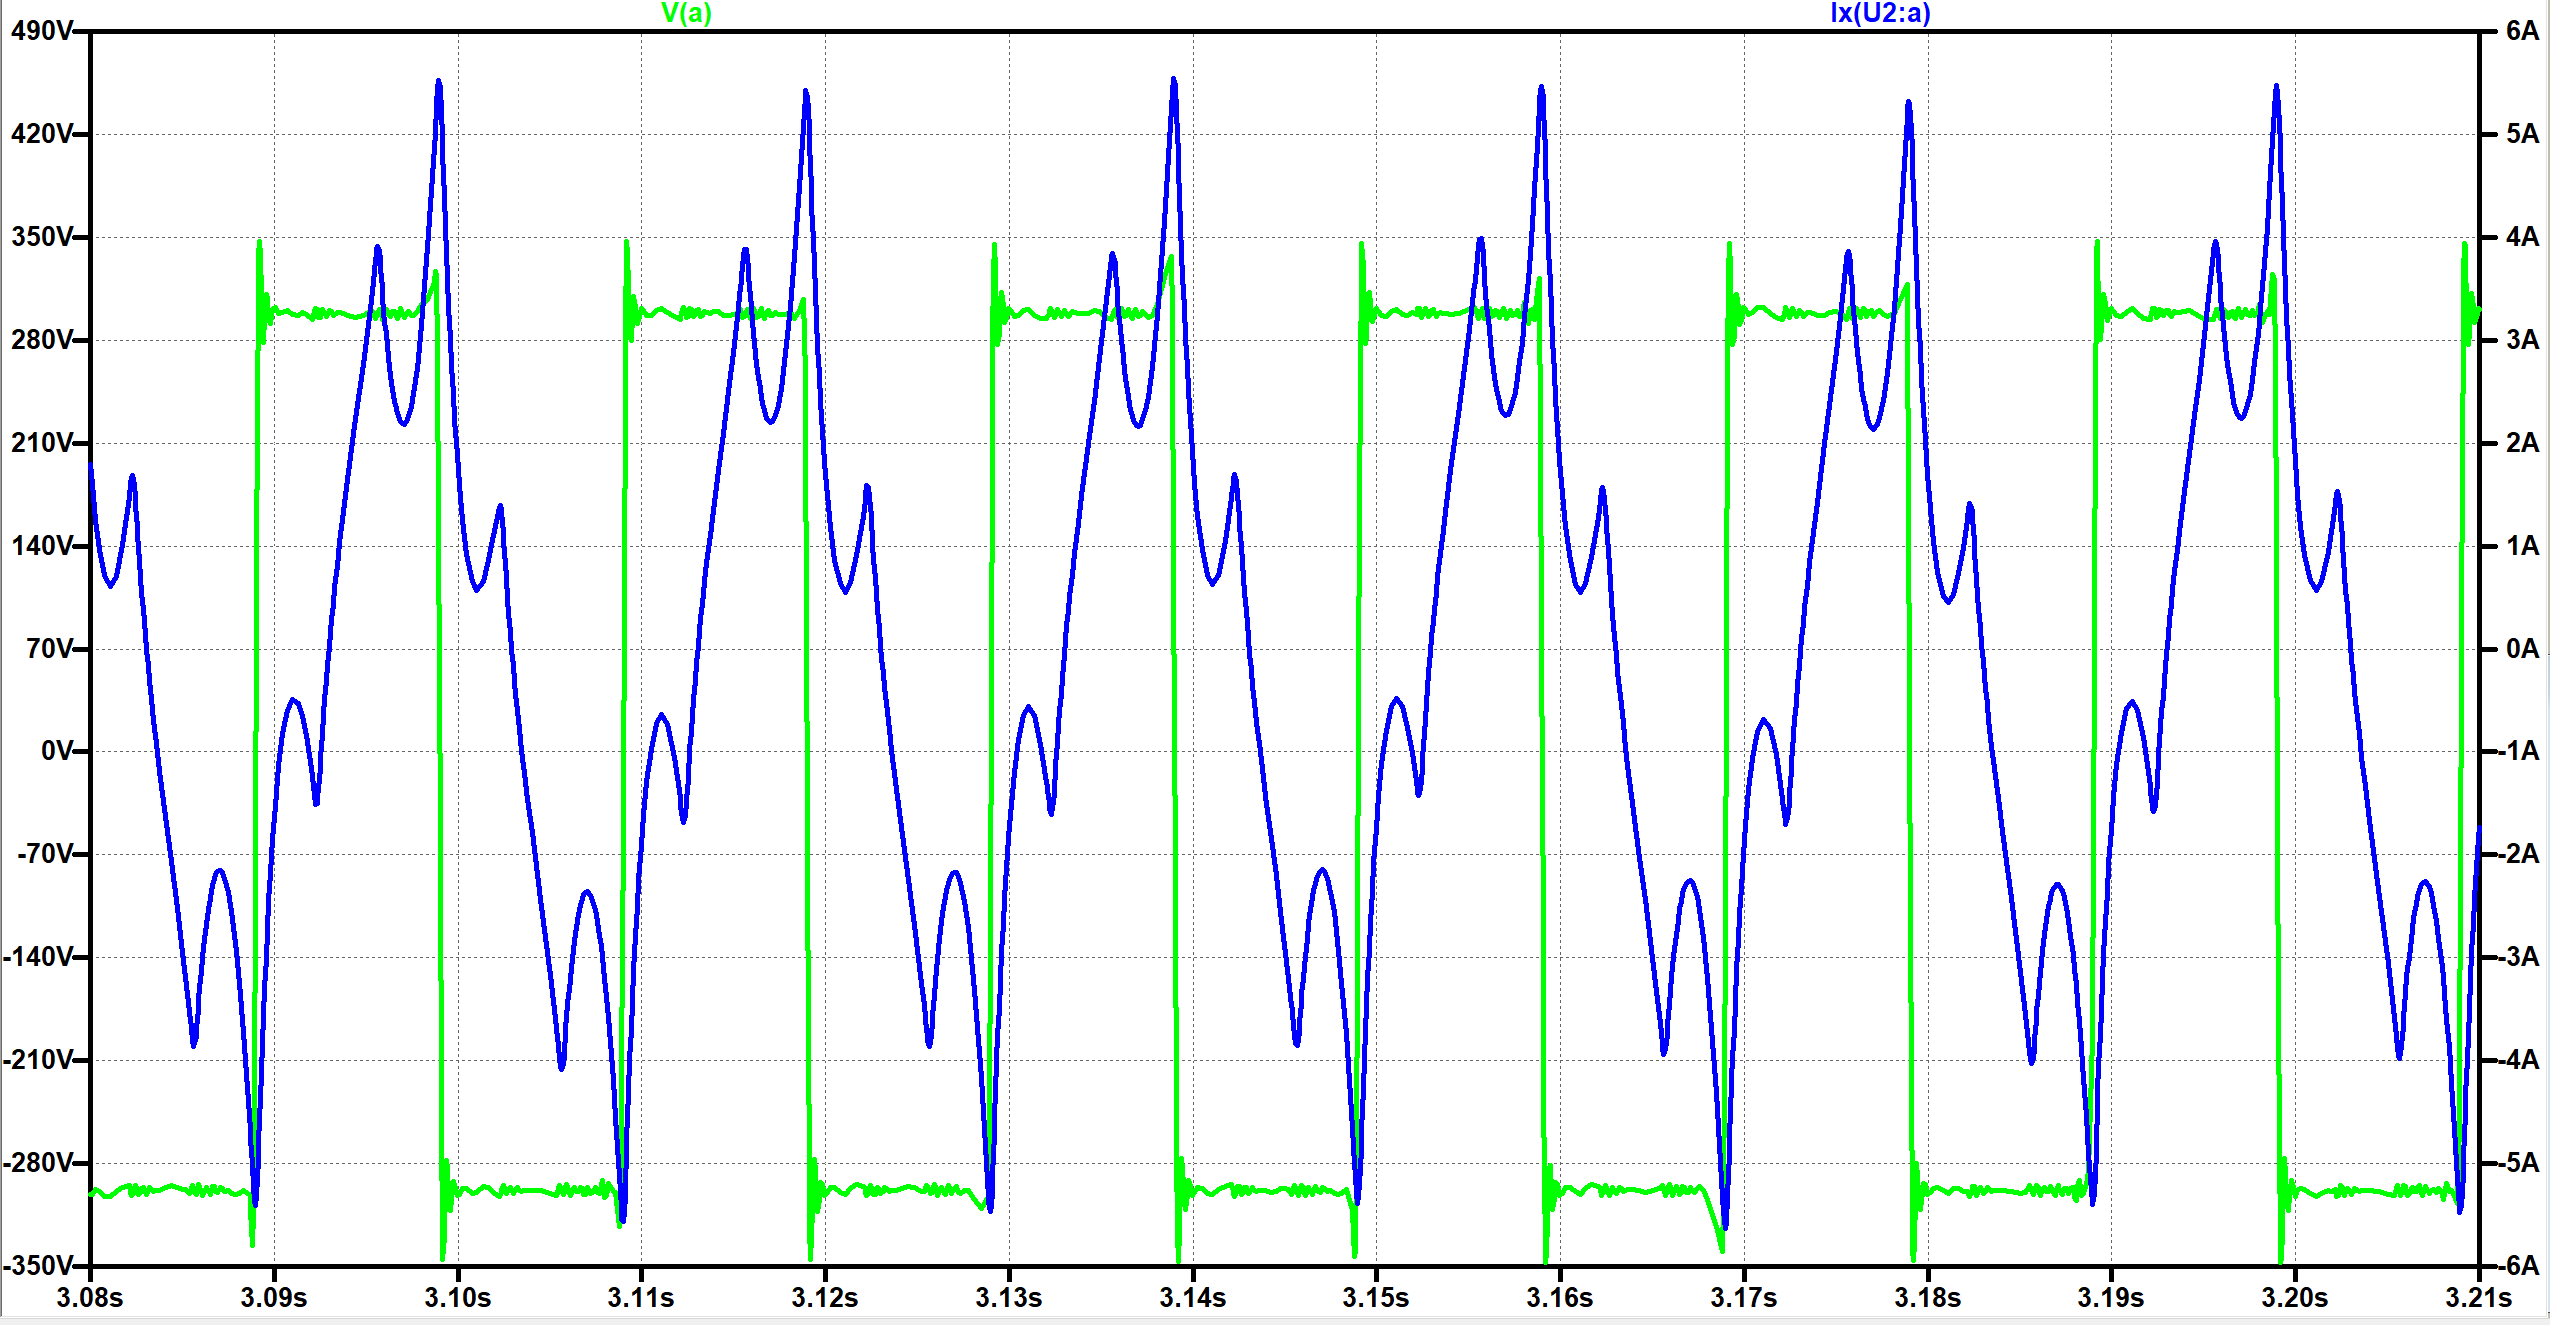
\includegraphics[width=0.9\linewidth]{Imagenes/3-1-a-linea.png}
    \caption{Tensi\'on de l\'inea y corriente de fase en b}
    \label{fig:f1}
  \end{subfigure}
  \hfill
  \begin{subfigure}[b]{0.49\textwidth}
  \centering
    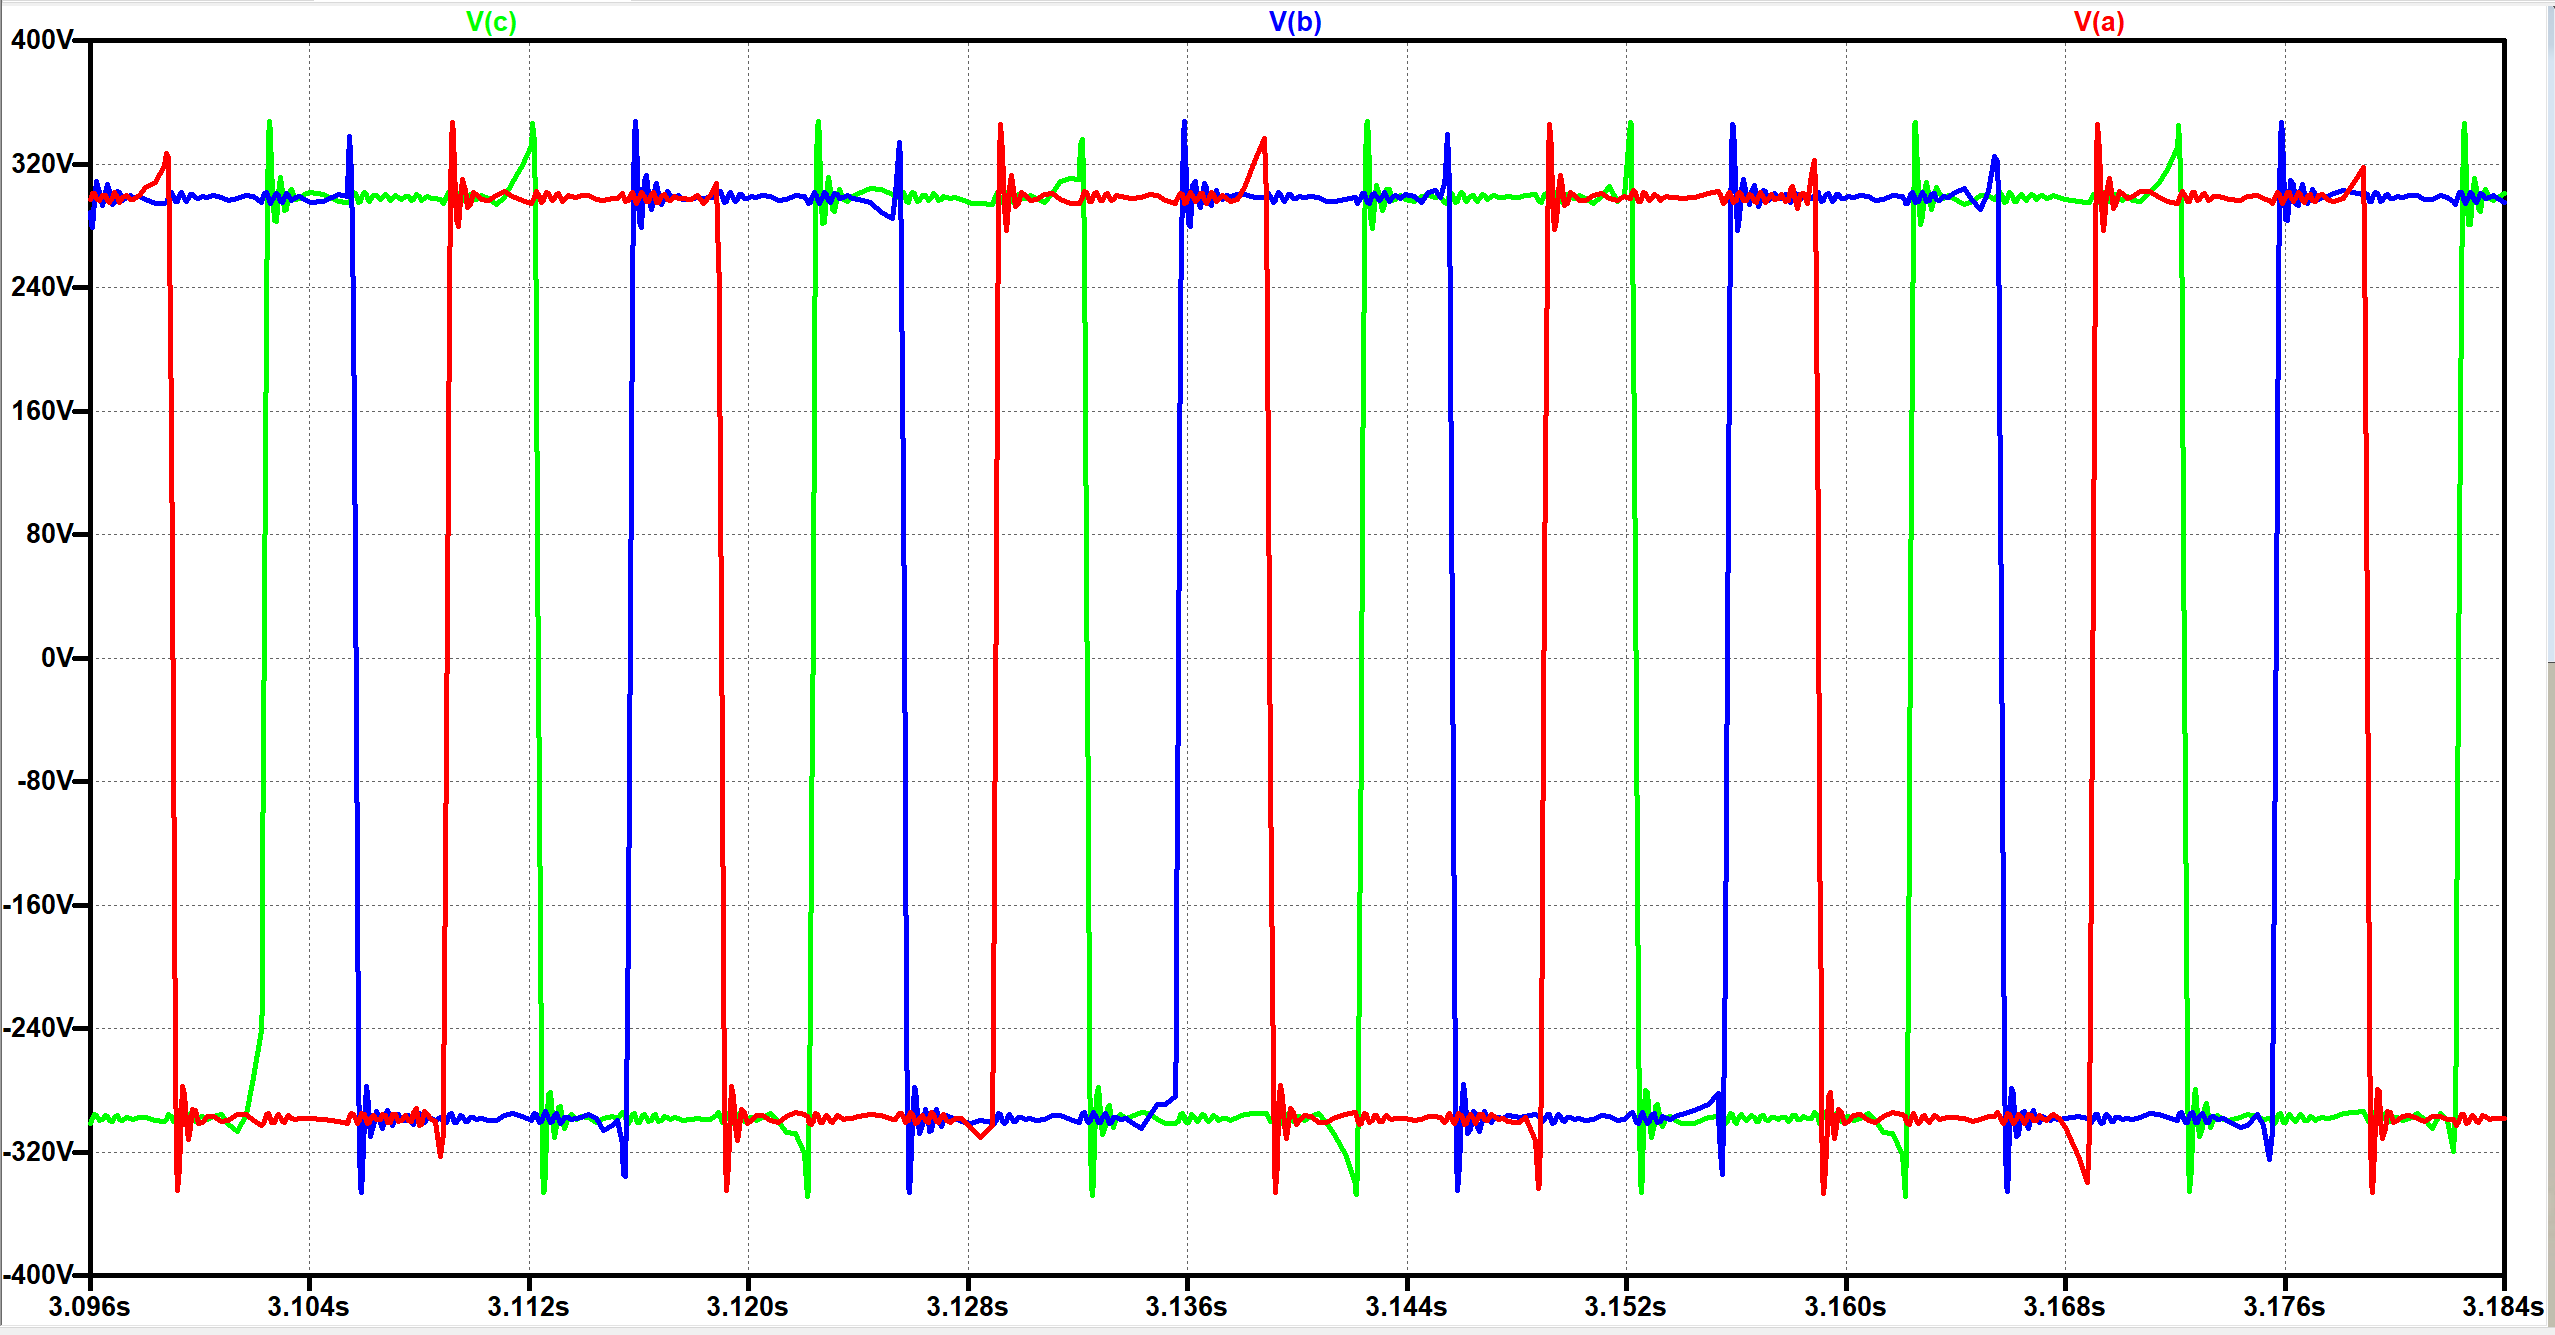
\includegraphics[width=0.9\linewidth]{Imagenes/3-1-a-lineas.png}
    \caption{Tensiones de l\'inea}
    \label{fig:f2}
  \end{subfigure}
  \caption{Corriente de fase y tensi\'on de l\'inea}
\end{figure}


Podemos observar que la tensión de línea tiene un valor de tensión $V_{RMS}=297.04V$, con picos de tensión de $V_{max}=345 V$ y una tensión $V_{on}=300V$. 
Las señales se encuentran desfazadas 120º entre sí, y la forma que poseen se debe a la presencia de armónicos. La fuente fue configurada para que entregue una señal con arm\'onicos impares.

Por otro lado, la corriente de fase tiene un valor de $I_{RMS}=2.59A$ , con picos de $I_{max}=5.4A$. 

\subsection{Análisis a lazo cerrado}
En esta etapa, vamos a realizar el análisis a lazo cerrado modificando el circuito como se encuentra en la consigna.

\begin{figure}[H]
	\centering
	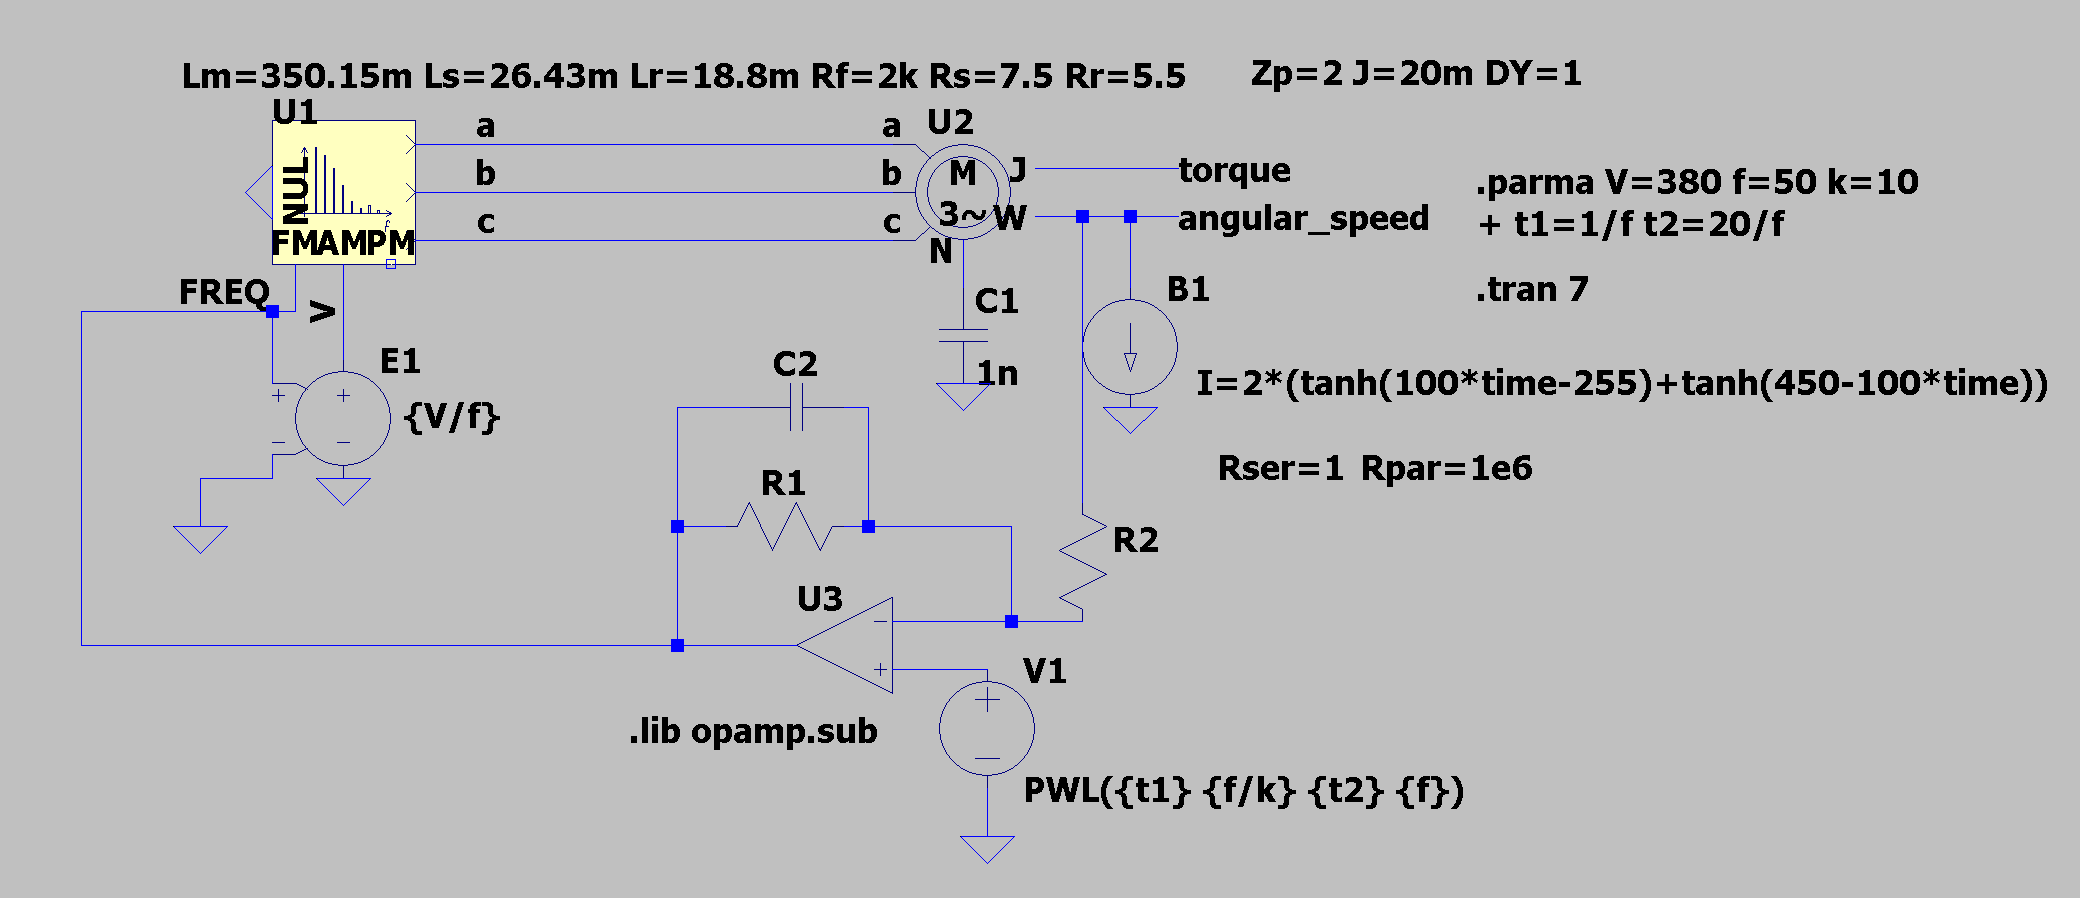
\includegraphics[width=0.7\linewidth]{Imagenes/3-2-circuito.png}
	\caption{Circuito realimentado}
	\label{fig:torq}
\end{figure}

Observamos que para cerrar el lazo, lo que tenemos que diseñar es un control PI (proporcional integrativo). La función transferencia de dicho PI es la siguiente:

$$\frac{V_o}{V_i}=-\frac{R_1}{R_2} \cdot \frac{1}{\$ R_1 C + 1} $$

Para lograr una respuesta sobreamortiguada sobre la velocidad angular se seleccionaron los valores:

 $$R1=R2=47k \Omega$$  
 $$C=4.7\mu$$

\vspace{5cm}
Al simular con dichos valores de componentes en LTSpice, se obtuvo el siguiente comportamiento del circuito realimentado. 

\begin{figure}[H]
	\centering
	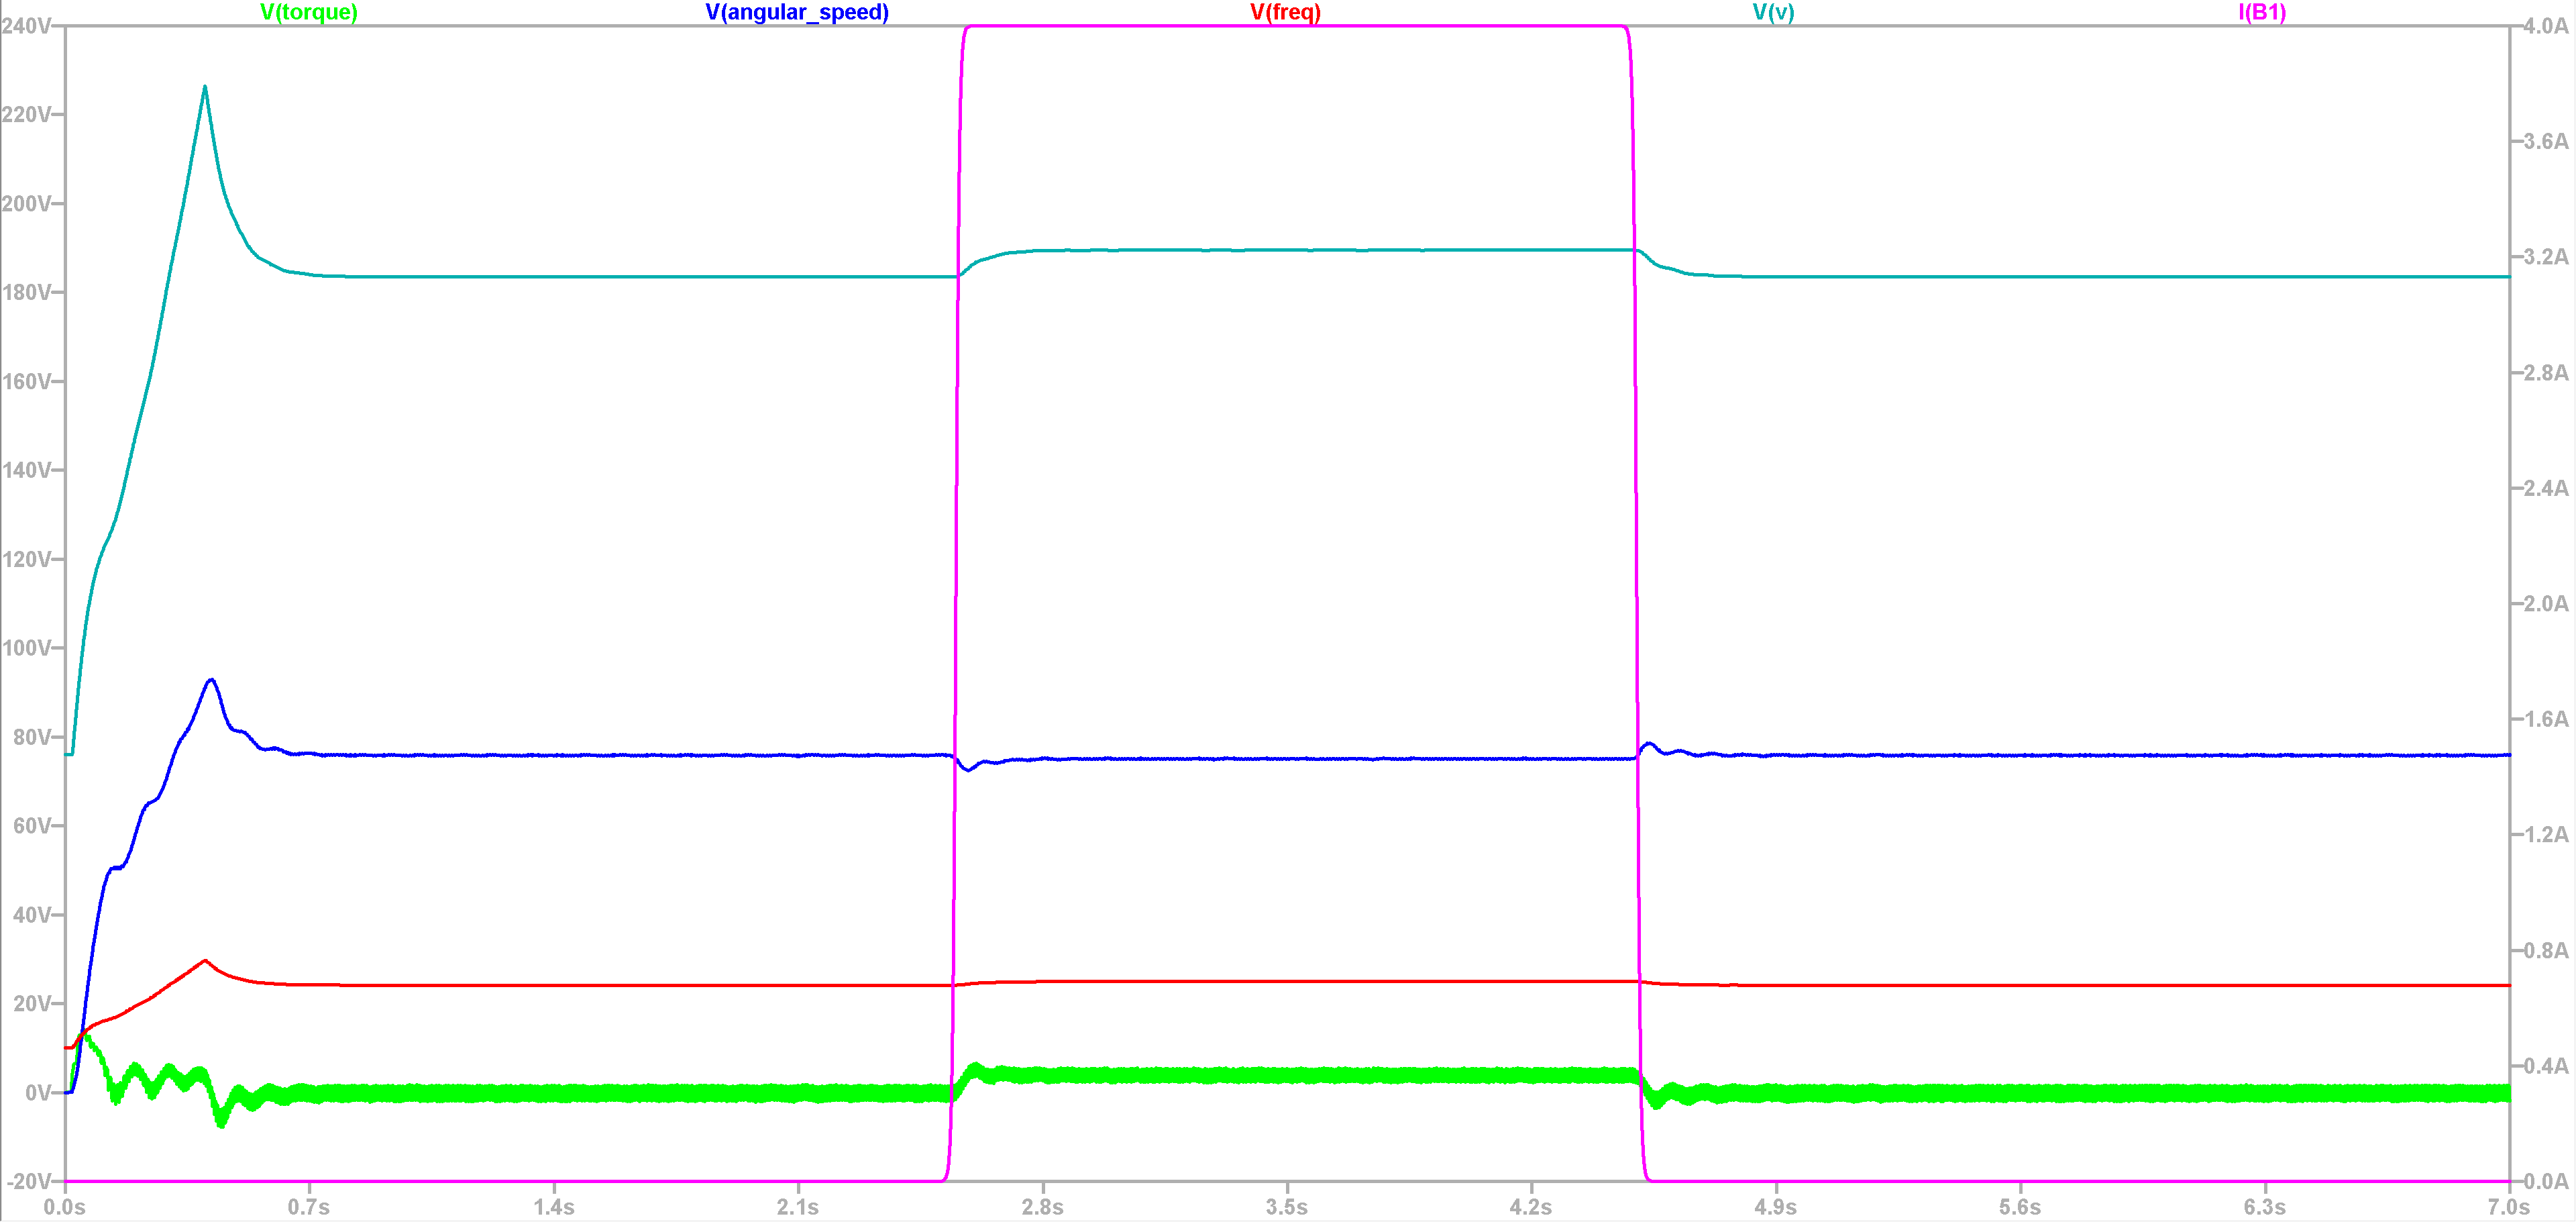
\includegraphics[width=0.8\linewidth]{Imagenes/3-2-subamortiguado.png}
	\caption{Simulación del circuito realimentado}
	\label{fig:torq}
\end{figure}


Lo que sucede ahora cuando se aplica el escal\'on de torque es que la velocidad angular cae por aproximadamente 120ms y luego vuelve a restablecerse al valor inicial. Lo mismo sucede cuando el escal\'on de torque cae: la velocidad angular aumenta unos milisegundos hasta que vuelve a su valor original. En ambos casos, lo hace con un comportamiento subamortiguado.  
\vspace{0.5cm}

Esto ocurre porque el circuito se encuentra realimentado, cuando ocurre un escal\'on de torque, la tensi\'on sobre el motor aumenta por lo que tambi\'en aumenta la frecuencia a la salida del inverter. En otras palabras, lo que esta sucediendo es que se esta corriendo la curva de torque del motor hacia la derecha. 

\end{document}

